\documentclass[11pt]{article}
\usepackage{fancyhdr}
\usepackage{geometry}
\usepackage{graphicx}
\usepackage{hyperref}
\usepackage[utf8]{inputenc}
\usepackage{lastpage}
\usepackage{xcolor}
\usepackage{amsmath}
\usepackage{amssymb}

% Fill these commands with right informations 
\newcommand{\SUBJECT}{...}
\newcommand{\TEACHER}{...}

% Dimension of pdf
\geometry{a4paper, top=1.5cm, bottom=1.5cm, left=1.5cm, right=1.5cm}

% Builder of header and footer
\fancypagestyle{plain}{
	\renewcommand{\headrulewidth}{0.4pt}
	\lhead{}
	\chead{\leftmark}
	\rhead{\thepage/\pageref{LastPage}}
	\renewcommand{\footrulewidth}{0.4pt} 
	\lfoot{\dag}
	\cfoot{Débruitage d'images par Analyse en Composantes Principales}
	\rfoot{\dag}
}
\pagestyle{fancy}
\renewcommand{\headrulewidth}{0.4pt}
\lhead{}
\chead{\leftmark}
\rhead{\thepage/\pageref{LastPage}}
\renewcommand{\footrulewidth}{0.4pt} 
\lfoot{\dag}
\cfoot{Débruitage d'images par Analyse en Composantes Principales}
\rfoot{\dag}
\definecolor{keywordcolor}{rgb}{0.13, 0.29, 0.53}
\definecolor{stringcolor}{rgb}{0.71, 0.18, 0.19}
\definecolor{commentcolor}{rgb}{0.2, 0.5, 0.2}
\definecolor{backgroundcolor}{rgb}{0.95, 0.95, 0.95}


% Hyperlink's color
\hypersetup{
    colorlinks=true,
    linkcolor=blue, 	% Intern color's color
    urlcolor=red    	% URL's color
}

% Import biblio
\usepackage[backend=biber, style=numeric, sorting=nyt]{biblatex}
\usepackage{csquotes} 
\addbibresource{content/biblio.bib}

% Active l'indentation des paragraphes (taille par défaut : 1.5em)
\usepackage{indentfirst} % Indente aussi le premier paragraphe après un titre
\setlength{\parindent}{1.5em} % Ajustez la taille de l'alinéa




\newcommand{\ABS}[1]{\LR{|}{#1}{|}}                         % mathmode              : absolute value
\newcommand{\BAN}[1]{\textlangle #1\textrangle}             % textmode              : between angle
\newcommand{\BAR}[1]{\overline{#1}}                         % mathmode              : a bar above a letter
\newcommand{\BBR}[1]{\LR{\{}{#1}{\}}}                       % mathmode              : between brackets
\newcommand{\BLR}[3]{\left#1 #2 \right#3}                   % mathmode              : between left right
\newcommand{\CAL}[1]{\mathcal{#1}}                          % mathmode {amssymb}    : caligraphic letter
\newcommand{\COV}[1]{\text{Cov}\LR{(}{#1}{)}}               % mathmode {amsmath}    : covariance 
\newcommand{\DIS}{\displaystyle}                            % mathmode              : displaystyle
\newcommand{\EPS}{\varepsilon}                              % mathmode {amsmath}    : epsilon
\newcommand{\EQU}{\Leftrightarrow}                          % mathmode              : equivalent arrow
\newcommand{\ESL}[1]{\mathscr{#1}}                          % mathmode {amssymb}    : elegant script letter
\newcommand{\EXP}[1]{\exp\LR{(}{#1}{)}}                     % mathmode {IDK}        : exponential
\newcommand{\FAM}[2]{\LR{(}{#1}{)}_{#2}}                    % mathmode              : family
\newcommand{\IINT}[2]{\iint_{#1}^{#2}}                      % mathmode              : double integral
\newcommand{\IND}{\perp \!\!\! \perp}                       % mathmode              : independant symbol
\newcommand{\IDC}[1]{\mathds{1}_{#1}}                       % mathmode {dsfont}     : indicator function
\newcommand{\INT}[2]{\int_{#1}^{#2}}                        % mathmode              : integral
\newcommand{\LIM}[1]{\underset{#1}{\text{lim}}}             % mathmode              : limit
\newcommand{\MAX}[1]{\underset{#1}{\text{max}}}             % mathmode              : max
\newcommand{\MIN}[1]{\underset{#1}{\text{min}}}             % mathmode              : min
\newcommand{\PTD}{\partial}                                 % mathmode              : partial derivate symbol
\newcommand{\RML}[1]{\mathrm{#1}}                           % mathmode {amssymb}    : roman letter
\newcommand{\SET}[1]{\mathbb{#1}}                           % mathmode {amssymb}    : set
\newcommand{\SETBT}[3]{\mathbb{#1}_{#2}^{#3}}               % mathmode {amssymb}    : set + bot and top 
\newcommand{\SUM}[2]{\sum_{#1}^{#2}}                        % mathmode              : sum
\newcommand{\TEN}[2]{\underset{#2}{\xrightarrow{#1}}}       % mathmode              : tend to
\newcommand{\TXT}[1]{\;\text{#1}\;}                         % mathmode {amsmath}    : insert text in math mode
\newcommand{\VEC}[1]{\overrightarrow{#1}}                   % mathmode              : vector

% Create a system with an #1 lines and arguments around it and possible commentary on right side
\newenvironment{SYSTEM}[1]{\begin{array}{r @{\quad #1 \quad} l l}}{\end{array}}


\begin{document}
\begin{titlepage}
    \begin{center}
        
\includegraphics[width=0.5\linewidth]{reference/picture/CYTECHlogo.png}\par\vspace{1cm}
        \vspace{0.5cm}
        {\huge \bfseries Situation d'apprentissage et d'évaluation : \par}
        {\huge \bfseries Débruitage d'images par Analyse en Composantes Principales \par}
    \end{center}
    \vspace{4cm}
    {\Large \textbf{CHOSSON} Clément\par}
    {\Large \textbf{GINESTE} Thomas \par}
    {\Large \textbf{MONDINA} Antonin \par}
    {\Large \textbf{THIEBAUT} Mattias \par}
    {\Large \textbf{VALENTE} Mathias \par}
    \vspace{0.5cm}
    {\large ING1 groupe 11 \par}
    \vspace{3cm}
    suppervisé par : RANISAVLJEVIC Élisabeth, \par
    \hspace{2.74cm}    
    FORTIN CAMDAVANT Nisrine, \par
    \hspace{2.74cm}    
    FASSI Dieudonné
    \vspace{4cm}
    \begin{center}
        25 mai 2025
    \end{center}
\end{titlepage}

\tableofcontents

\setlength{\headheight}{14.5pt}.
\addtolength{\topmargin}{-1.6pt}

% Section 1 : Introduction
\newpage
\section{Introduction} 

contexte du projet en 1 ou 2 paragraphe

\paragraph{Problématique}
expliquer la Problématique

\paragraph{Objectifs}
expliquer les Objectifs

\paragraph{Organisation}
expliquer l'organisation et le déroulé du rapport

% Section 2 : Solutions au problème
\newpage
\section{Réponses au problème}

\subsection{Approche mathématiques}
\subsubsection{Préambule}
Pour commencer nos explications, nous allons démontrer que l'on peut décomposer un vecteur \(V\) correspondant à un patch dans une base orthonormée.\newline
\begin{figure}[hbt!]
    Soit \(\beta = \{u_{1}, \ldots, u_{s^{2}}\}\) une base orthonormée de \(\mathbb{R}^{s^{2}}\).\\
On notera ici \(u\) un vecteur de \(\beta\) et \(u^{\top}\) sa transposée. \\

Soit \(x = V(k) - m(v) \in \mathbb{R}^{s^{2}}\).

On a :
\[
x = \sum_{i=1}^{s^{2}} \beta_{i} u_{i}
\]

De plus :
\[
\langle x \mid u_{j} \rangle = \left\langle \sum_{i=1}^{s^{2}} \beta_{i} u_{i} \big{|} u_{j} \right\rangle = \sum_{i=1}^{s^{2}} \beta_{i} \langle u_{i} \mid u_{j} \rangle = \beta_{j} \langle u_{j} \mid u_{j} \rangle = \beta_{j}
\]

Donc :
\[
\beta_{i} = \langle x \mid u_{i} \rangle
\]

Ainsi :
\[
V(k) - m(v) = \sum_{i=1}^{s^{2}} \langle V(k) - m(v) \mid u_{i} \rangle \, u_{i} = \sum_{i=1}^{s^{2}} u_{i}^{\top} \left( V(k) - m(v) \right) u_{i}
\]

Finalement :
\[
V(k) = m(v) + \sum_{i=1}^{s^{2}} u_{i}^{\top} \left( V(k) - m(v) \right) u_{i}
\]
    \caption{Démonstration de la décomposition de V dans une base orthonormée}
\end{figure}

\subsection{Transformation du problème en mathématiques}
Tout d'abord, l'objectifs du débruitage est de travailler sur des patchs qui sont des petits carrées de pixels extraient de l'image. Nous allons représenter ces patchs en noir et blanc comme un vecteur dont le valeurs sont dans \([0,255]\). Les s pixels de la première ligne seront les s premiers du vecteurs, ainsi de suite. \par
Nous allons ensuite faire ressortir le bruit à l'aide de l'ACP appliqué sur ces vecteurs. L'ACP va dé-corréler les variables, ce qui va centrer les variables importantes, et rendre abérantes les varibales de bruits. \par
En appliquants un seuillage avec une valeur seuil, nous pourrons supprimer les variables abérantes, et donc supprimer le bruit.

\subsection{Approche informatique}
Comme demandé, notre application permettant de répondre à cette problématique de bruitage est développé en Java et l'interface graphique à l'aide de JavaFX. \par
Pour ce qui est de la structure du code, nous avons divisé le problème en plusieurs classes

\subsection{Choix initiaux}
Justifier notre livrable 1 et dire ce que nous avons changé

% Section 3 : Présentation de l'interfaces graphiques
\newpage
\section{Présentation de notre interface utilisateur}

\subsection{Présentation DA}
Présenter la fenêtre en général, ses différentes zones, \dots

\subsection{Justification}
On explique pourquoi on a mit un slider, un bouton, affiché ça \dots

% Section 4 : Présentation des résultats obtenus
\newpage
\section{Présentation des résultats}
\subsection{Préambule}
Dans tout ce projet, nous avions 3 indicateurs afin de déterminer la qualité de notre débruitage :
\subsubsection{MSE} 
Il mesure la différence moyenne au carré entre l'image originale (de référence) et l'image débruitée.
 \[
    \TXT{MSE}= \dfrac{1}{lc}\SUM{i=1}{l}\SUM{j=1}{c}\BLR{(}{X(i,j)-Y(i,j)}{)}^2
 \]
 avec \(X\) l'image bruité et \(Y\) l'image débruité, \((l,c)\) le nombre de lignes et colonnes et \((i,j)\) la position des pixels. \par
 Pour son interprétation, un MSE\(=0\) signifie que les deux images sont identiques et plus il est élevé, plus l'image débruité est dégradée
 \subsubsection{PSNR}
 Le PSNR (en dB) compare le signal maximal possible (valeur maximale d'un pixel, dans notre cas 255) au bruit (erreur mesurée par le MSE).
 \[
    \TXT{PSNR}=10\cdot\log_{10}\BLR{(}{\dfrac{255^2}{\TXT{MSE}}}{)}
 \]
Pour son interprétation, on suit les règles suivantes :
\begin{itemize}
    \item inférieur à 20 dB : qualité médiocre
    \item entre 30 dB et 40 dB : qualité acceptable voire bonne
    \item supérieur à 40 dB : très bonne qualité
\end{itemize}

\subsubsection{Amélioration}
Il s'agit d'une variable que nous avons ajouté et qui permet de définir un pourcentage d'amélioration en suivant la formule suivante :
\[
    \TXT{amelioration} = \dfrac{\TXT{mseBruitee} - \TXT{mse}}{\TXT{mseBruitee}}*100
\]
 
\subsection{Valeur idéale de taille de patch}

Dans un premier temps, nous avons cherché à déterminer quelle était la taille optimale de patch pour obtenir les meilleures performances de débruitage. La table ci-dessous présente les résultats obtenus avec une méthode globale, un seuillage dur et un seuil de type VisuShrink (sigma = 20, image Lena).

\begin{table}[hbt!]
    \centering
    \begin{tabular}{|l|l|l|l|}
    \hline
        Taille du patch & MSE & PSNR & Amélioration \\ \hline
        5x5 & 48.20 & 31.30 & 87.92 \%\\ \hline
        6x6 & 43.34 & 31.76 & 89.14 \%\\ \hline
        7x7 & 41.27 & 31.97 & 89.66 \%\\ \hline
        8x8 & 40.52 & 32.05 & 89.85 \%\\ \hline
        9x9 & 40.66 & 32.04 & 89.81 \%\\ \hline
        10x10 & 41.17 & 31.98 & 89.68 \%\\ \hline
        11x11 & 41.55 & 31.94 & 89.59 \%\\ \hline
        12x12 & 42.26 & 31.87 & 89.41 \%\\ \hline
    \end{tabular}
    \caption{Valeurs de performances selon la taille des patchs}
\end{table}

On observe que la performance augmente avec la taille du patch jusqu’à 8x8, puis se stabilise, voire régresse légèrement. La taille 8x8 fournit le meilleur compromis, avec une MSE minimale (40.52) et un PSNR maximal (32.05 dB). Cette taille offre donc une couverture spatiale suffisante pour l’ACP tout en évitant de mélanger des zones trop hétérogènes.


\subsection{Limites de notre programme}

Nous avons ensuite évalué les limites de notre programme du point de vue des temps d'exécution, en faisant varier la taille de l'image d'entrée. Le tableau ci-dessous indique le temps total nécessaire pour effectuer les 8 méthodes de débruitage, pour un niveau de bruit de $\sigma = 25$.

\begin{table}[hbt!]
    \centering
    \begin{tabular}{|l|c|c|c|c|}
    \hline
        Taille de l'image & 128x128 & 256x256 & 512x512 & 1024x1024 \\ \hline
        Temps d’exécution & 1,2 s & 3,5 s & 11,4 s & 43,3 s \\ \hline
    \end{tabular}
    \caption{Temps d’exécution selon la taille de l'image}
\end{table}

On constate une croissance quasi-exponentielle du temps d'exécution avec la taille de l’image. Cette tendance est attendue, car une image plus grande implique un plus grand nombre de pixels, donc un plus grand nombre de patchs à extraire, projeter, seuiller et reconstruire. Cette complexité s'applique pour chacune des 8 méthodes, expliquant les temps cumulés observés.


\subsection{Détermination de la meilleure méthode}

Enfin, nous avons comparé les 8 combinaisons possibles de méthode de seuillage (doux ou dur), calcul de seuil (VisuShrink ou BayesShrink), et mode d’ACP (global ou local). Les résultats suivants ont été obtenus sur l’image Lena bruitée avec $\sigma = 25$, en utilisant des patchs 8x8.

\begin{table}[hbt!]
    \centering
    \begin{tabular}{|l|l|l|l|}
    \hline
        Méthode utilisée & MSE & PSNR & Amélioration \\ \hline
        Global/Doux/Visu & 246.55 & 24.21 & 44.26 \%\\ \hline
        Global/Doux/Bayes & 212.78 & 24.85 & 51.90 \%  \\ \hline
        Global/Dur/Visu & 87.89 & 28.69 & 80.13 \% \\ \hline
        Global/Dur/Bayes & 421.16 & 21.89 & 4.79 \% \\ \hline
        Local/Doux/Visu & 243.26 & 24.27 & 45.01 \% \\ \hline
        Local/Doux/Bayes & 202.40 & 25.07 & 54.24 \%\\ \hline
        Local/Dur/Visu & 87.04 & 28.73 & 80.32 \% \\ \hline
        Local/Dur/Bayes & 416.45 & 21.94 & 5.85 \% \\ \hline
    \end{tabular}
    \caption{Performances des différentes méthodes}
\end{table}

L'analyse des résultats montre clairement que les méthodes utilisant un seuillage dur couplé à VisuShrink (en global ou local) offrent les meilleurs scores en MSE et PSNR, avec environ 80\% d'amélioration. La meilleure méthode est Local/Dur/Visu avec une MSE de 87.04 et un PSNR de 28.73 dB.

Les méthodes utilisant BayesShrink en combinaison avec un seuillage dur donnent au contraire les pires performances, ce qui s'explique par une estimation de seuil trop faible et une élimination excessive du signal utile.

Les variantes douces (soft) donnent des résultats intermédiaires, avec un meilleur équilibre entre atténuation du bruit et conservation des détails.

On retiendra donc que la meilleure méthode sur cette image est celle utilisant un seuillage dur avec VisuShrink, en ACP locale.\par
En annexe (\ref{fig:lenaSource}), vous trouverez un de nos résultats pour la méthode Global/Dur/Visu sur l'image Lena.


% Section 5 : Conclusion
\newpage
\section{Conclusion}
On peut conclure en nuançant nos résultats, disant que ce n'est pas la meilleure methode, ect \dots

% Section 6 : Annexes
\newpage
\section{Annexes}

\begin{figure}[hbt!]
    \centering
    
\includegraphics[width=0.35\linewidth]{reference/picture/lenaSource.png}
    \caption{Lena (image source)}
    \label{fig:lenaSource}
\end{figure}

\begin{figure}[hbt!]
    \centering
    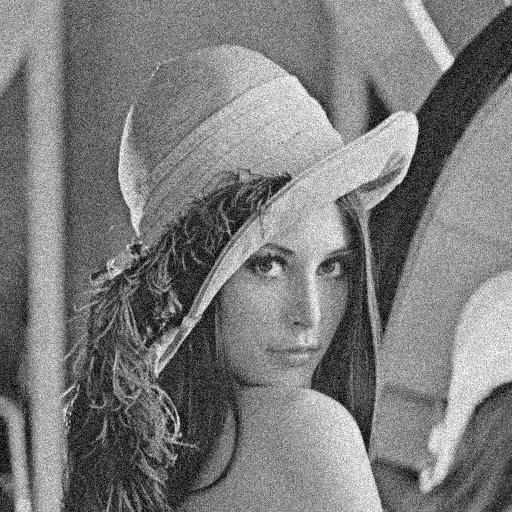
\includegraphics[width=0.35\linewidth]{reference/picture/lenaNoised.png}
    \caption{Lena (image bruité : sigma = 20)}
\end{figure}
\begin{figure}[hbt!]
    \centering
    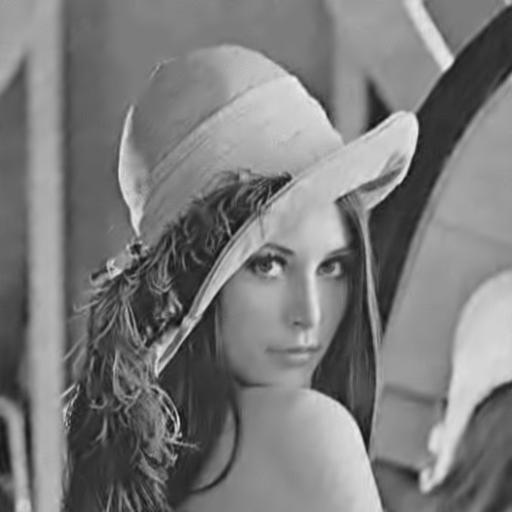
\includegraphics[width=0.35\linewidth]{reference/picture/lenaDenoised.png}
    \caption{Lena (image débruité (Global/Dur/Visu))}
\end{figure}

 \begin{figure}[hbt!]
     \centering
     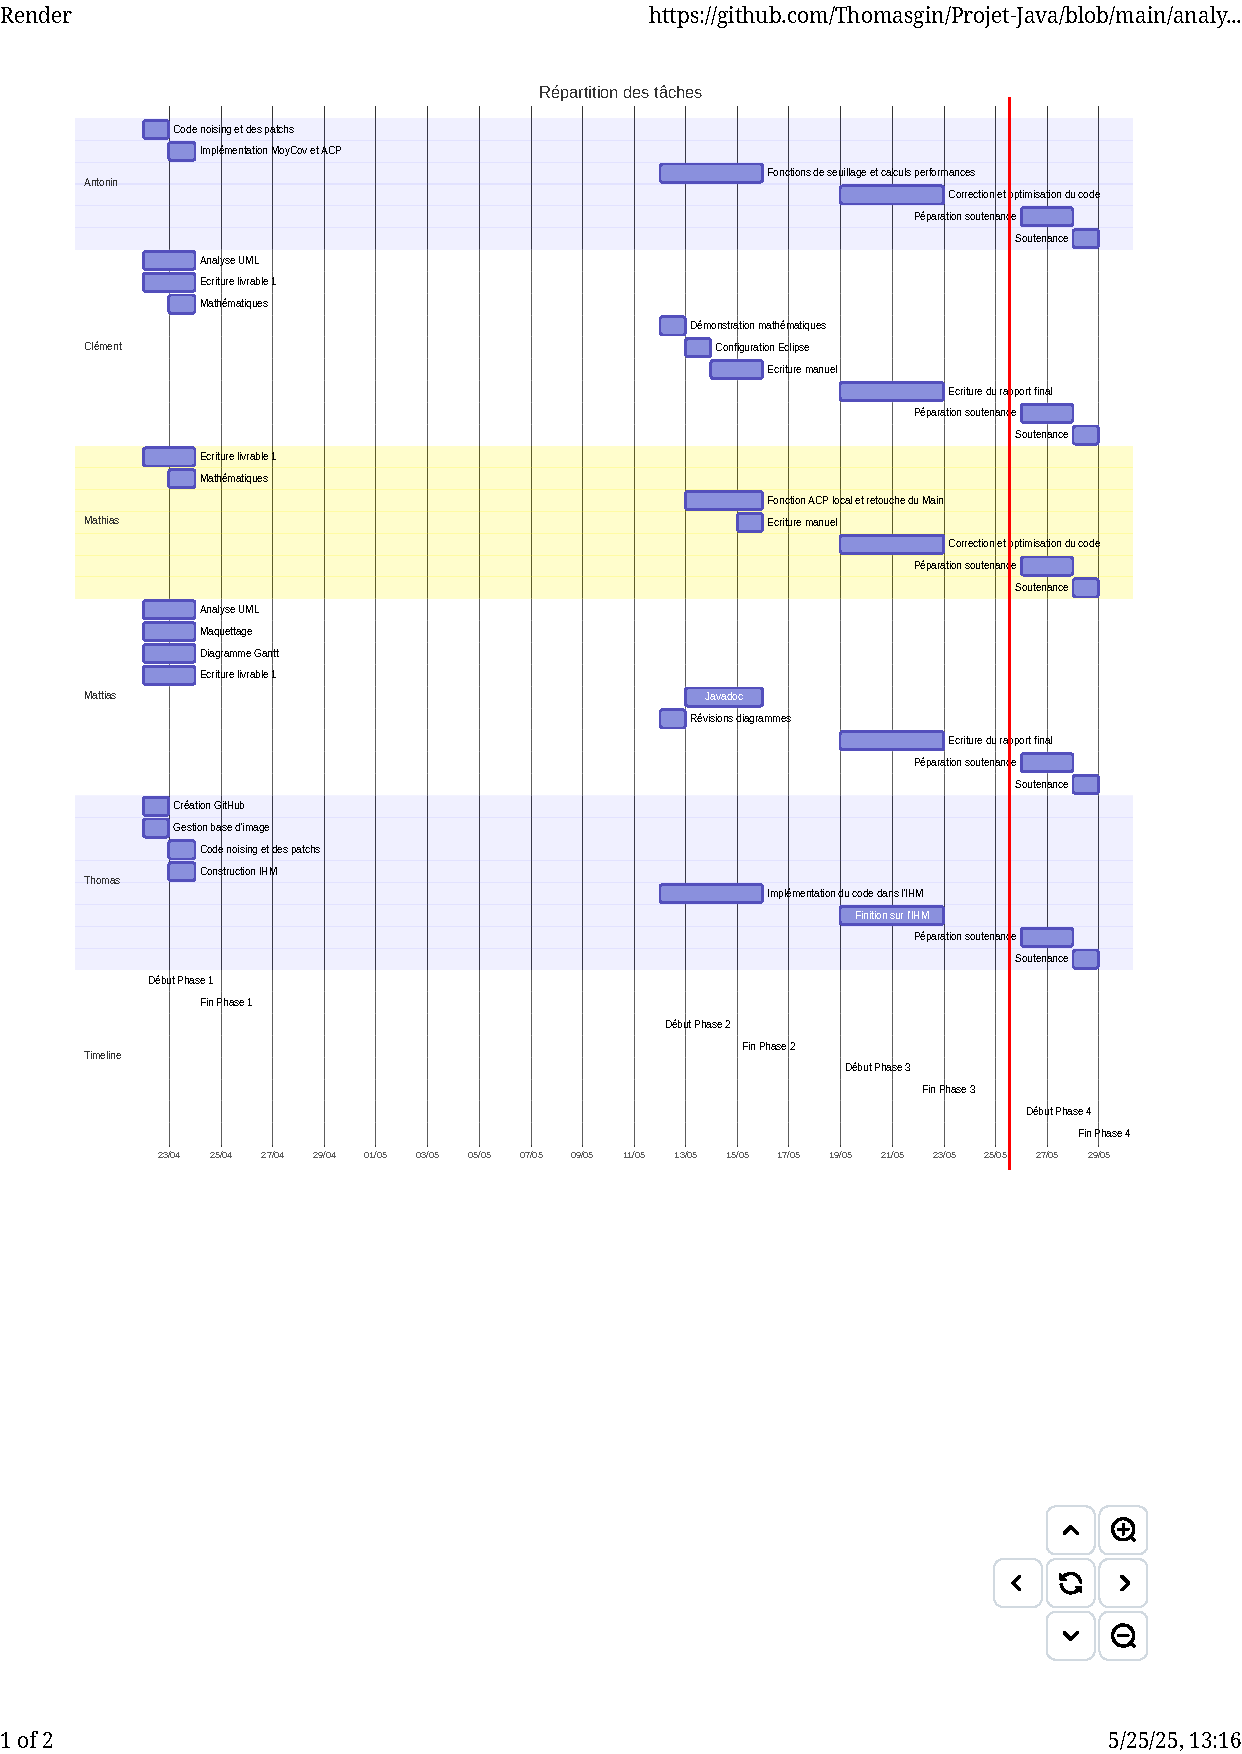
\includegraphics[page=1, trim=1cm 10cm 1cm 1cm, clip, width=1\linewidth]{reference/diagram/ganttTemp.pdf}
     \caption{Diagramme de Gantt}
     \label{fig:gantt}
 \end{figure}




% Bibliographie
\newpage
\nocite{*}
\null \newpage
\printbibliography[title={Références}]
\end{document}